%% -----------------------------------------
\Section{Experiments}
\label{section:experiments}

We present a few examples on which we applied the method. As the
equivalent petri net for each example can quickly grow, we narrowed
down the examples to a characteristic part, namely to test the
presence or absence of data races. Some examples are classical
examples of synchronization disciplines. We implemented a small
prototype in Java and report in table~\ref{table:experiments} the
results of the runs. We display the number of configurations kept at
any time in the analysis (\#Conf.), the number of configurations that
have been subsumed (\#Subsum., i.e.\ discarded by the algorithm
because already simulated by other smaller configurations), and the
number of iteration of the algorithm (\#Iter.). Note that we also
tested some examples that did contain a data race. We also added
whether the analysis found a race or not. All examples ran in less
than a second\footnote{ Performance is not exactly the focus in this
  paper, nor are limitations, but we wanted to show that it was not a
  bottleneck.}.

\begin{figure}
  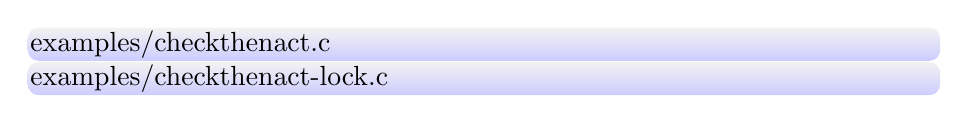
\begin{tikzpicture}
    [every node/.append style={rounded corners,inner sep=1pt,bottom color=blue!20,top color=gray!10!white}]
    \node[text width=0.95\linewidth,above] (cta) {\lstinputlisting{examples/checkthenact.c}};
    \node[text width=0.95\linewidth,below] (cta2){\lstinputlisting{examples/checkthenact-lock.c}};
  \end{tikzpicture}
  \caption{Check then act in pthreaded code. The read in the if statement was not ``secured''.}
  \label{fig:checkthenact}
\end{figure}

The \verb+Counter+ and \verb+CounterWithLock+ examples represent a
shared counter which is incremented as depicted in
Figure~\ref{fig:languageExampleCS}. The \verb+CheckThenAct+ and
\verb+CheckThenAct-Lock+ examples represent a classical race condition
described in Section~\ref{section:introduction} and depicted in
Figure~\ref{fig:checkthenact}.
%
Figure~\ref{fig:languageExampleProdsCons} depicts the
\verb+Prods/Cons+ (\verb+Prods/Cons 2+ is another variant) as the
classical producer/consumer programming style.
%
Note that the \verb+Lock-ReadWriteOnly+ example shows a program that
secures only the read and write accesses to shared variable. A thread
in that program can indeed read a shared variable, store it in a local
variable, change the local variable as it wishes, and store the result
back into the shared variable. While there is no data race in that
program, it is not a good programming practice, as the shared variable
might have been updated, and the first read of the shared variable
does not reflect its actual value. It has indeed been argued
in~\cite{FQ03} that the absence of data race is not a strong enough
condition.

% \begin{figure}
%   \begin{tikzpicture}
%     [every node/.append style={rounded corners,inner sep=1pt,bottom color=blue!20,top color=gray!10!white}]
%     \node[text width=0.5\linewidth,below left] (l) {\lstinputlisting{examples/onlyLockingReadWriteAccesses.c}};
%     \node[text width=0.5\linewidth,below right] (r) {\lstinputlisting{examples/onlyLockingReadWriteAccesses-sml.c}};
%   \end{tikzpicture}
%   \caption{Only locking the read and write accesses for a shared variable.}
%   \label{fig:checkthenact}
% \end{figure}

\begin{table}
{\footnotesize
\caption{Experimental Results}
\label{table:experiments}
\centering
\begin{tabular}{|l|c|c|c|c|}\hhline{*{5}{=}}
  {\bf Prog.}    & {\bf \#Conf.} & {\bf \#Subsum.} & {\bf \#Iter.} & {\bf Safe?}\\\hhline{*{5}{=}}
  \verb+Counter+                   & 10 & 3 & 4 & - \\\hline
  \verb+CounterWithLock+           & 14 & 7 & 6 & \checkmark \\\hline
  \verb+CheckThenAct+              & 20 & 12 & 5 & - \\\hline
  \verb+CheckThenAct-Lock+      & 13 & 4 & 4 & \checkmark \\\hline
  \verb+Prods/Cons+       & 310 & 645 & 19 & \checkmark \\\hline
  \verb+Prods/Cons 2+     & 290 & 561 & 17 & \checkmark \\\hline
  \verb+Lock-ReadWriteOnly+ & 25 & 13 & 8 & \checkmark\\\hhline{*{5}{=}}
\end{tabular}
}
\end{table}
